% =============================================================================
%  CHAPITRE 3 : PRÉSENTATION DU SITE DE L'ÉTUDE, DES DONNÉES ET DES RÉSULTATS
%
%  Structure imposée par le « Guide de rédaction KEYCE v3.0 » (§ 13 et § 14) :
%      Introduction
%      3.1. Présentation du site de l'étude
%      3.2. Présentation des données et des résultats
%      Conclusion
% =============================================================================
\entete{Chapitre 3 : Site de l'étude, données et résultats}
\chapter{Présentation du site de l'étude, des données et des résultats}
\label{chap:terrain}

\introchap

Ce chapitre confronte au terrain la démarche exposée précédemment. Il présente
d'abord le site de l'étude, c'est-à-dire la Fondation Jean Félicien Gacha et
son Département \emph{Think Tank} Fou'ndjem, qui nous a accueilli. Il expose
ensuite les données recueillies auprès du personnel et des visiteurs,
l'implémentation du dispositif construit à partir de ces données, puis les
résultats obtenus. La présentation reste ici factuelle : son interprétation au
regard des hypothèses de l'étude est réservée au chapitre~\ref{chap:diagnostic}.

% =============================================================================
\section{Présentation du site de l'étude}
\label{sec:site}

\subsection{Identification de la structure}

La Fondation Jean Félicien Gacha est une organisation à but non lucratif de
droit camerounais implantée à Bangoulap, dans l'arrondissement de Bangangté,
département du Ndé, région de l'Ouest du Cameroun. Elle intervient dans la
culture, l'art, l'artisanat, l'éducation et le développement communautaire. Le
tableau~\ref{tab:fiche} en présente la fiche d'identification.

\begin{table}[!ht]
\centering
\caption{Fiche d'identification de la Fondation Jean Félicien Gacha}
\label{tab:fiche}
\small
\begin{tabularx}{\textwidth}{|L{5.2cm}|X|}
\hline
\rowcolor{keycetete}
\thead{Désignation} & \thead{Affectation} \\ \hline
Dénomination & Fondation Jean Félicien Gacha \\ \hline
Nature juridique & Fondation, organisation à but non lucratif \\ \hline
Secteur d'activité & Culture, art, artisanat, éducation, développement communautaire \\ \hline
Siège & Bangoulap, arrondissement de Bangangté, département du Ndé, région de l'Ouest \\ \hline
Pays & Cameroun \\ \hline
% À COMPLÉTER AVANT REMISE (exigé par le guide, § 13) : décommenter et renseigner.
% Date de création & \dots \\ \hline
% Effectif du personnel & \dots \\ \hline
Domaines d'intervention & Espaces d'exposition, ateliers de création, résidences d'artistes, espaces verts, actions communautaires \\ \hline
Entité d'accueil du stage & Département \emph{Think Tank} Fou'ndjem \\ \hline
Encadreur professionnel & M. Adrien GHOMSI \\ \hline
Période du stage & Du 20 juin au 20 août 2026 \\ \hline
\end{tabularx}
\source{Documents internes de la Fondation et entretiens, juin 2026.}
\end{table}

Deux éléments de cette fiche commandent la suite du travail : la Fondation
détient un patrimoine exposé sur un site unique, dont la découverte suppose un
déplacement ; et l'entité qui nous a accueilli n'est pas un service
d'exploitation, mais un département de réflexion.

\subsection{Historique, missions et organisation}

La Fondation porte le nom de son initiateur, Jean Félicien Gacha, dont l'action
visait à faire de Bangoulap un lieu de rencontre entre la création
contemporaine et les savoir-faire hérités des chefferies de l'Ouest. Née d'une
initiative privée, la structure s'est progressivement dotée d'espaces
d'exposition, d'ateliers et de résidences, puis a élargi son action au
développement communautaire : sa trajectoire va de la collection privée à
l'institution ouverte au public, puis à l'acteur du développement territorial.
Elle explique le trait saillant du terrain sur lequel s'appuie toute notre
intervention : un patrimoine matériel et documentaire considérable, mais une
organisation encore fondée sur la mémoire des personnes et sur des supports non
structurés.

Ses missions se regroupent en quatre ensembles : \textbf{conserver et présenter}
le patrimoine de l'Ouest camerounais ; \textbf{soutenir la création}, par
l'accueil d'artistes en résidence ; \textbf{transmettre}, envers les scolaires,
les chercheurs et les visiteurs ; et contribuer au \textbf{développement
communautaire} local.

Sur le plan organisationnel, la Fondation est administrée par un conseil
d'administration et dirigée par une direction générale, assistée d'un
secrétariat général. Cinq départements se partagent l'activité : le
\textbf{Département Scolaire}, dont relève l'\textbf{ISBB}, l'établissement
d'enseignement de la Fondation ; le \textbf{Département Culture et patrimoine},
qui a la charge des espaces d'exposition et des collections ; le
\textbf{Département Artisanat et création}, qui accueille les ateliers et les
résidences d'artistes ; le \textbf{Département Développement communautaire},
dont dépendent l'accueil du public et la communication ; et le
\textbf{Département Administration et finances}. Le \emph{Think Tank}
Fou'ndjem constitue le dernier département : structure de réflexion et de
recherche, il ne conduit aucune activité opérationnelle et n'exerce aucune
autorité sur les autres. La figure~\ref{fig:organigramme} en donne la
représentation.

\begin{figure}[!ht]
\centering
\schema{organigramme}
\caption{Organigramme de la Fondation Jean Félicien Gacha}
\label{fig:organigramme}
\source{Élaboré par nos soins à partir des entretiens conduits en juin 2026.}
\end{figure}


\subsection{Le Département \emph{Think Tank} Fou'ndjem et son rôle dans le projet}
\label{sec:thinktank}

Le Département \emph{Think Tank} Fou'ndjem est la structure de la Fondation
dédiée à la réflexion et à la recherche sur le Cameroun, sa culture, son
patrimoine et son développement : un espace de veille et d'analyse où sont
examinées les problématiques contemporaines susceptibles d'éclairer les grands
enjeux du pays, notamment celles qui touchent à la modernisation des
infrastructures et au développement technologique.

C'est dans ce cadre que le Département nous a accueilli. Son rôle n'a pas été
celui d'un client opérationnel : il n'administre pas les collections, ne reçoit
pas le public et n'est pas l'utilisateur final de la plateforme, fonctions qui
relèvent des pôles Conservation et exposition, Accueil du public et
Communication. Il a tenu celui d'un cadre d'encadrement intellectuel et
méthodologique, notre encadreur, M. Adrien GHOMSI, nous ayant proposé de faire
mûrir un thème initialement esquissé pour en faire un sujet de fin d'études
aligné sur notre spécialité en génie informatique.

Notre travail a dès lors consisté à contextualiser cette réflexion : concevoir
une plateforme de valorisation numérique du patrimoine adaptée aux réalités
camerounaises — connectivité mobile instable, coût des données, sécurité en
environnement multi-institutions. Ces trois contraintes ne sont pas restées
théoriques : elles ont commandé la priorité donnée au téléphone mobile, la
sobriété des médias transportés et le cloisonnement des données par
institution, décrits à la section~\ref{sec:implementation}.

Le tableau~\ref{tab:entites} situe les entités concernées
et distingue le cadre d'accueil du périmètre d'application : le Département a
cadré et validé la question de recherche en nous laissant la liberté
méthodologique de la traiter, tandis que les pôles opérationnels ont fourni la
matière documentaire et constituent les utilisateurs finaux du dispositif. Cette
distinction écarte un contresens fréquent, qui consisterait à prendre l'entité
d'accueil pour le commanditaire fonctionnel.

\begin{table}[!ht]
\centering
\caption{Entités de la Fondation concernées par l'étude}
\label{tab:entites}
\small
\begin{tabularx}{\textwidth}{|L{3.6cm}|L{4.4cm}|X|}
\hline
\rowcolor{keycetete}
\thead{Entité} & \thead{Rôle dans l'organisation} & \thead{Lien avec l'étude} \\ \hline
Direction & Conduite de la Fondation & Ouverture des espaces et des archives ; validation du principe du projet \\ \hline
Département \emph{Think Tank} Fou'ndjem & Réflexion, veille et recherche sur le patrimoine et le développement & Structure d'accueil du stage ; cadrage intellectuel et méthodologique du sujet \\ \hline
Pôle Conservation et exposition & Collections, salles et notices & Source de la matière documentaire ; utilisateur final du back-office \\ \hline
Pôle Accueil du public & Visites guidées, entrées, ventes d'artisanat & Terrain d'observation ; utilisateur final de la boutique en ligne \\ \hline
Pôle Communication & Présence en ligne de la Fondation & Utilisateur final du site public et des campagnes d'information \\ \hline
\end{tabularx}
\source{Élaboré par nos soins à partir des entretiens conduits en juin 2026.}
\end{table}

\subsection{Environnement technologique existant}

La Fondation n'abordait pas le numérique en terrain vierge : une première
version en ligne existait déjà, et c'est d'elle qu'il faut partir. Cette version
présentait des \textbf{photographies d'œuvres et d'objets}, chacune suivie d'une
\textbf{brève description} textuelle. Le travail engagé n'est donc pas une
informatisation à partir de rien, mais la transformation d'une vitrine en un
dispositif de médiation.

Le relevé conduit durant la première semaine du stage précise ce que cette
version permettait et ce qu'elle ne permettait pas. Elle donnait à voir les
pièces, mais \textbf{sans parcours} : les photographies se consultaient une à
une, sans qu'aucun cheminement ne relie les espaces entre eux, et sans que le
visiteur puisse examiner un objet sous tous ses angles ni en apprécier la taille.
Elle décrivait chaque pièce, mais \textbf{sans possibilité d'interrogation}.
C'est le manque le plus lourd, et il mérite d'être chiffré : un visiteur qui
voulait en savoir davantage sur une matière, une technique ou une histoire
n'avait d'autre recours que d'écrire à la Fondation, et la réponse mettait
\textbf{de dix à vingt jours} à lui parvenir lorsqu'elle lui parvenait, une part
des demandes restant sans réponse. Un tel délai n'est pas une lenteur
administrative : il annule la question, car le visiteur a cessé d'attendre bien
avant. C'est cette constatation qui a rendu l'assistant conversationnel
\textbf{crucial} plutôt qu'accessoire.

La version en ligne présentait enfin les objets isolément, \textbf{sans mise en
relation} avec les collections d'autres institutions, et ne s'accompagnait
\textbf{d'aucun outil de gestion} : les descriptions étaient saisies dans les
pages elles-mêmes, sans inventaire structuré derrière, de sorte que toute mise à
jour supposait une intervention technique.

Ce sont ces quatre manques, et non une absence de présence numérique, qui
constituent la valeur de départ à laquelle seront comparées, au
tableau~
ef{tab:mesures}, les valeurs relevées après mise en service.


\subsection{Cadre et déroulement du stage}
\label{sec:stage}

Le stage s'est déroulé du 20 juin au 20 août 2026. Il a débuté par un entretien
avec M. Adrien GHOMSI, consacré aux attentes de la structure et aux objectifs de
la période, puis par une visite complète des espaces conduite par le pôle
Accueil du public, qui nous a permis de prendre la mesure du lieu, condition
préalable à toute tentative de le restituer numériquement, et d'observer dès la
première semaine des visites guidées réelles ainsi que les questions que les
visiteurs y posent spontanément. Les travaux ont ensuite suivi le programme
hebdomadaire présenté au tableau~\ref{tab:chronogramme}
dont l'économie est la suivante : trois semaines de terrain et de cadrage, six
semaines de réalisation menées par ordre de priorité décroissante des attentes
recueillies, une dernière semaine d'industrialisation, de mise en ligne et de
mesure.

\begin{table}[!ht]
\centering
\caption{Chronogramme des tâches effectuées durant le stage}
\label{tab:chronogramme}
\footnotesize
\begin{tabularx}{\textwidth}{|L{3.4cm}|X|}
\hline
\rowcolor{keycetete}
\thead{Période} & \thead{Tâches effectuées} \\ \hline
Du 20 au 26 juin 2026 &
Accueil et présentation de la Fondation ; prise de contact avec le personnel du
Département \emph{Think Tank} Fou'ndjem ; visite complète des espaces ; cadrage
du sujet avec l'encadreur professionnel ; observation de visites guidées. \\ \hline
Du 27 juin au 3 juillet 2026 &
Étude de l'existant ; entretiens semi-directifs avec six membres du personnel ;
relevé de l'environnement numérique ; dépouillement des inventaires et des
notices ; administration du questionnaire aux visiteurs. \\ \hline
Du 4 au 10 juillet 2026 &
Rédaction du cahier des charges ; arbitrage des besoins avec l'encadreur
professionnel ; choix de l'architecture et des technologies. \\ \hline
Du 11 au 17 juillet 2026 &
Conception et création de la base de données ; mise en place du cloisonnement
par organisation ; développement du back-office : musées, salles, œuvres,
tarifs, médias. \\ \hline
Du 18 au 24 juillet 2026 &
Développement du site public ; catalogue, fiches d'œuvres, boutique,
gestion des événements et du livre d'or. \\ \hline
Du 25 au 31 juillet 2026 &
Développement du moteur de visite immersive à 360~degrés ; éditeur de parcours
dans le back-office ; pose des points d'intérêt ; enchaînement des salles. \\ \hline
Du 1\textsuperscript{er} au 7 août 2026 &
Numérisation en trois dimensions ; réalité augmentée ; génération des codes QR ;
essais de photogrammétrie et d'acquisition par capteur LiDAR ; couverture des
appareils Android et iOS. \\ \hline
Du 8 au 14 août 2026 &
Développement de l'assistant conversationnel à ancrage documentaire ;
rapprochement documentaire avec les collections ouvertes ; module de généalogie ;
campagnes d'information aux adhérents. \\ \hline
Du 15 au 20 août 2026 &
Conteneurisation ; chaînes d'intégration et de déploiement continus ;
description de l'infrastructure ; mise en ligne ; essais de bout en bout ;
mesures de performance et de coût ; restitution à l'encadreur professionnel. \\ \hline
\end{tabularx}
\source{Journal de bord du stage, juin--août 2026.}
\end{table}

\paragraph{Justification du choix du terrain.} Trois caractéristiques font de
ce terrain un cas instructif : une richesse patrimoniale réelle et documentée,
qui écarte le risque de construire un dispositif sans matière ; des contraintes
de moyens représentatives de celles des institutions patrimoniales de la
sous-région, de sorte que ce qui fonctionne ici a des chances de fonctionner
ailleurs ; et un interlocuteur, le Département \emph{Think Tank} Fou'ndjem,
capable de formuler le besoin et d'arbitrer les choix, condition indispensable à
une recherche interactive.

% =============================================================================
\section{Présentation des données et des résultats}
\label{sec:donnees}

\subsection{Les données recueillies}

\subsubsection{Étude de l'existant}

L'étude de l'existant identifie les forces, les faiblesses et les besoins non
satisfaits du dispositif en place. Le tableau~\ref{tab:existant} récapitule les
insuffisances relevées et les besoins qu'elles induisent.

\begin{table}[!ht]
\centering
\caption{Insuffisances du dispositif existant et besoins induits}
\label{tab:existant}
\small
\begin{tabularx}{\textwidth}{|L{4.4cm}|X|L{3.4cm}|}
\hline
\rowcolor{keycetete}
\thead{Domaine} & \thead{Insuffisance constatée} & \thead{Besoin induit} \\ \hline
Accès au lieu & La visite exige un déplacement physique & Parcours immersif à distance \\ \hline
Perception des œuvres et des espaces & Photographies plates suivies d'une brève description & Visite à 360	extdegree{}, présentation en 3D, espaces en réalité augmentée \\ \hline
Documentation & Notices dispersées, objets traités isolément & Inventaire structuré et mise en relation \\ \hline
Information du visiteur & Question adressée par courriel, réponse en 10 à 20 jours ou sans suite & Assistant conversationnel ancré sur les documents \\ \hline
Gestion administrative & Registres papier, données non sauvegardées & Progiciel de gestion intégré \\ \hline
Relation au public & Aucun fichier de visiteurs & Adhésion en ligne et campagnes d'information \\ \hline
Rayonnement & Dispositif non transposable à d'autres institutions & Architecture ouverte à plusieurs organisations \\ \hline
\end{tabularx}
\source{Étude de l'existant, juin--juillet 2026.}
\end{table}

Chaque insuffisance appelle un besoin précis, et chacun de ces besoins se
retrouve plus loin sous la forme d'une fonctionnalité livrée. Les sept lignes
couvrent l'accès, la perception, la documentation, l'information du visiteur, la
gestion, la relation au public et le rayonnement : le déficit n'est pas
ponctuel, il est systémique.

\subsubsection{Résultats du questionnaire}

Le questionnaire a été administré à 42 visiteurs. Le
tableau~\ref{tab:profil} présente le profil des
répondants ; le tableau~\ref{tab:attentes} ci-après expose leurs attentes.

\begin{table}[!ht]
\centering
\caption{Profil des répondants au questionnaire}
\label{tab:profil}
\small
\begin{tabularx}{\textwidth}{|L{4.0cm}|X|C{2.2cm}|C{2.2cm}|}
\hline
\rowcolor{keycetete}
\thead{Caractéristique} & \thead{Modalité} & \thead{Effectif} & \thead{Fréquence} \\ \hline
\multirow{3}{*}{Tranche d'âge}
 & 18 à 30 ans & 19 & 45,2 \% \\ \cline{2-4}
& 31 à 45 ans & 15 & 35,7 \% \\ \cline{2-4}
& 46 ans et plus & 08 & 19,1 \% \\ \hline
\multirow{3}{*}{Provenance}
 & Région de l'Ouest & 21 & 50,0 \% \\ \cline{2-4}
& Autre région du Cameroun & 14 & 33,3 \% \\ \cline{2-4}
& Étranger & 07 & 16,7 \% \\ \hline
\multirow{2}{*}{Équipement principal}
 & Téléphone mobile & 36 & 85,7 \% \\ \cline{2-4}
& Ordinateur & 06 & 14,3 \% \\ \hline
\rowcolor{keycetotal}
\textbf{Total} & & \textbf{42} & \textbf{100 \%} \\ \hline
\end{tabularx}
\source{Enquête par questionnaire, juillet 2026.}
\end{table}

Deux enseignements ressortent de ce profil. D'une part, la moitié des visiteurs
vient déjà de l'extérieur de la région, ce qui atteste l'existence d'un public
prêt à s'intéresser à la Fondation à distance. D'autre part, plus de huit
visiteurs sur dix accèdent au numérique par un téléphone mobile : le dispositif
devait donc être conçu pour le téléphone en priorité, et non pour l'ordinateur.

\begin{table}[!ht]
\centering
\caption{Attentes exprimées à l'égard d'un dispositif de visite à distance}
\label{tab:attentes}
\small
\begin{tabularx}{\textwidth}{|X|C{2.4cm}|C{2.4cm}|}
\hline
\rowcolor{keycetete}
\thead{Attente exprimée} & \thead{Effectif} & \thead{Fréquence} \\ \hline
Se déplacer dans les salles comme si l'on y était & 38 & 90,5 \% \\ \hline
Voir les objets sous tous leurs angles et connaître leur taille réelle & 35 & 83,3 \% \\ \hline
Poser des questions et obtenir une réponse immédiate & 33 & 78,6 \% \\ \hline
Savoir à qui l'objet a appartenu et d'où il vient & 29 & 69,0 \% \\ \hline
Savoir si des objets semblables existent ailleurs dans le monde & 24 & 57,1 \% \\ \hline
Acheter un billet ou un objet d'artisanat en ligne & 18 & 42,9 \% \\ \hline
\end{tabularx}
\source{Enquête par questionnaire, juillet 2026, questions à réponses multiples.}
\end{table}

Ces résultats confirment la hiérarchie retenue dans les objectifs : la
restitution du déplacement dans l'espace arrive en tête, suivie de la perception
des objets, puis de la possibilité d'interroger. Ils valident également la
pertinence de la mise en relation entre institutions, souhaitée par plus d'un
visiteur sur deux alors même qu'elle ne figurait pas dans la demande initiale.

\subsection{L'implémentation du système}
\label{sec:implementation}

\subsubsection{Architecture générale de la plateforme}

L'architecture retenue comporte trois couches. Une \textbf{couche de
présentation} s'exécute dans le navigateur du visiteur : elle regroupe le site
public, le back-office et les moteurs de rendu écrits sur mesure. Une
\textbf{couche de services} regroupe la base de données, l'authentification et
douze fonctions serveur qui exécutent tout ce qui exige une clé d'accès ou un
privilège. Une \textbf{couche de diffusion} sert les fichiers statiques depuis
un réseau de distribution mondial.

Le principe directeur est simple et n'a jamais été enfreint : \emph{aucune clé
d'accès à un service tiers ne se trouve dans le navigateur}. Toute demande
adressée à un modèle de langue, à un service de synthèse vocale ou à un service
de paiement transite par une fonction serveur qui détient seule le secret.

\begin{figure}[!ht]
\centering
\schema{architecture-generale}
\caption{Architecture générale de la plateforme MUSÉA}
\label{fig:archi}
\source{Élaboré par nos soins.}
\end{figure}

\subsubsection{Architecture de l'assistant conversationnel à ancrage documentaire}

L'assistant repose sur une architecture de génération augmentée par la
recherche, dont le principe a été exposé au chapitre~1. Sa mise en œuvre suit
cinq temps.

\begin{enumerate}
  \item \textbf{Ingestion.} Les documents de référence de la Fondation (notices d'œuvres, descriptions de salles, histoires des musées,
        biographies des personnages, foire aux questions) sont exportés depuis
        la base de données et déposés dans un espace de stockage d'objets. Ce
        dépôt constitue la source de vérité documentaire : rien de ce qui n'y
        figure pas ne peut fonder une réponse.

  \item \textbf{Découpage et vectorisation.} Chaque document est découpé en
        fragments de taille homogène, puis converti en vecteur numérique par un
        modèle de plongement. Un point de méthode s'est révélé décisif : les
        fragments sont plongés \textbf{en anglais}. Les mesures conduites
        montrent en effet qu'une requête française classait une peinture sans
        rapport devant deux masques réellement apparentés, tandis qu'en anglais
        les correspondances légitimes atteignaient un score d'au moins 0,898
        contre au plus 0,779 pour le bruit, une étendue de 0,20 contre 0,13.

  \item \textbf{Indexation.} Les vecteurs sont enregistrés dans la base de
        données, dans une colonne vectorielle de dimension 384 dotée d'un index
        de type HNSW en distance cosinus. Cet index rend la recherche des plus
        proches voisins praticable sans parcourir l'ensemble des fragments.

  \item \textbf{Recherche et augmentation.} À la réception d'une question, la
        fonction serveur applique d'abord ses garde-fous : elle répond avec
        courtoisie aux salutations, refuse poliment les sujets hors périmètre,
        et restreint le cas échéant la recherche au musée ou à la salle où se
        trouve le visiteur. Elle convertit ensuite la question en vecteur,
        récupère les fragments les plus proches et compose l'instruction
        adressée au modèle de langue.

  \item \textbf{Génération contrôlée.} Le modèle rédige la réponse. La consigne
        lui interdit d'énoncer un fait absent des fragments fournis, lui impose
        de citer l'institution et le numéro d'inventaire lorsqu'ils existent, et
        l'autorise explicitement à déclarer qu'aucune conclusion n'est possible.
        Cette autorisation est essentielle : sans elle, un modèle de langue
        préfère inventer plutôt que de décevoir.
\end{enumerate}

\begin{figure}[!ht]
\centering
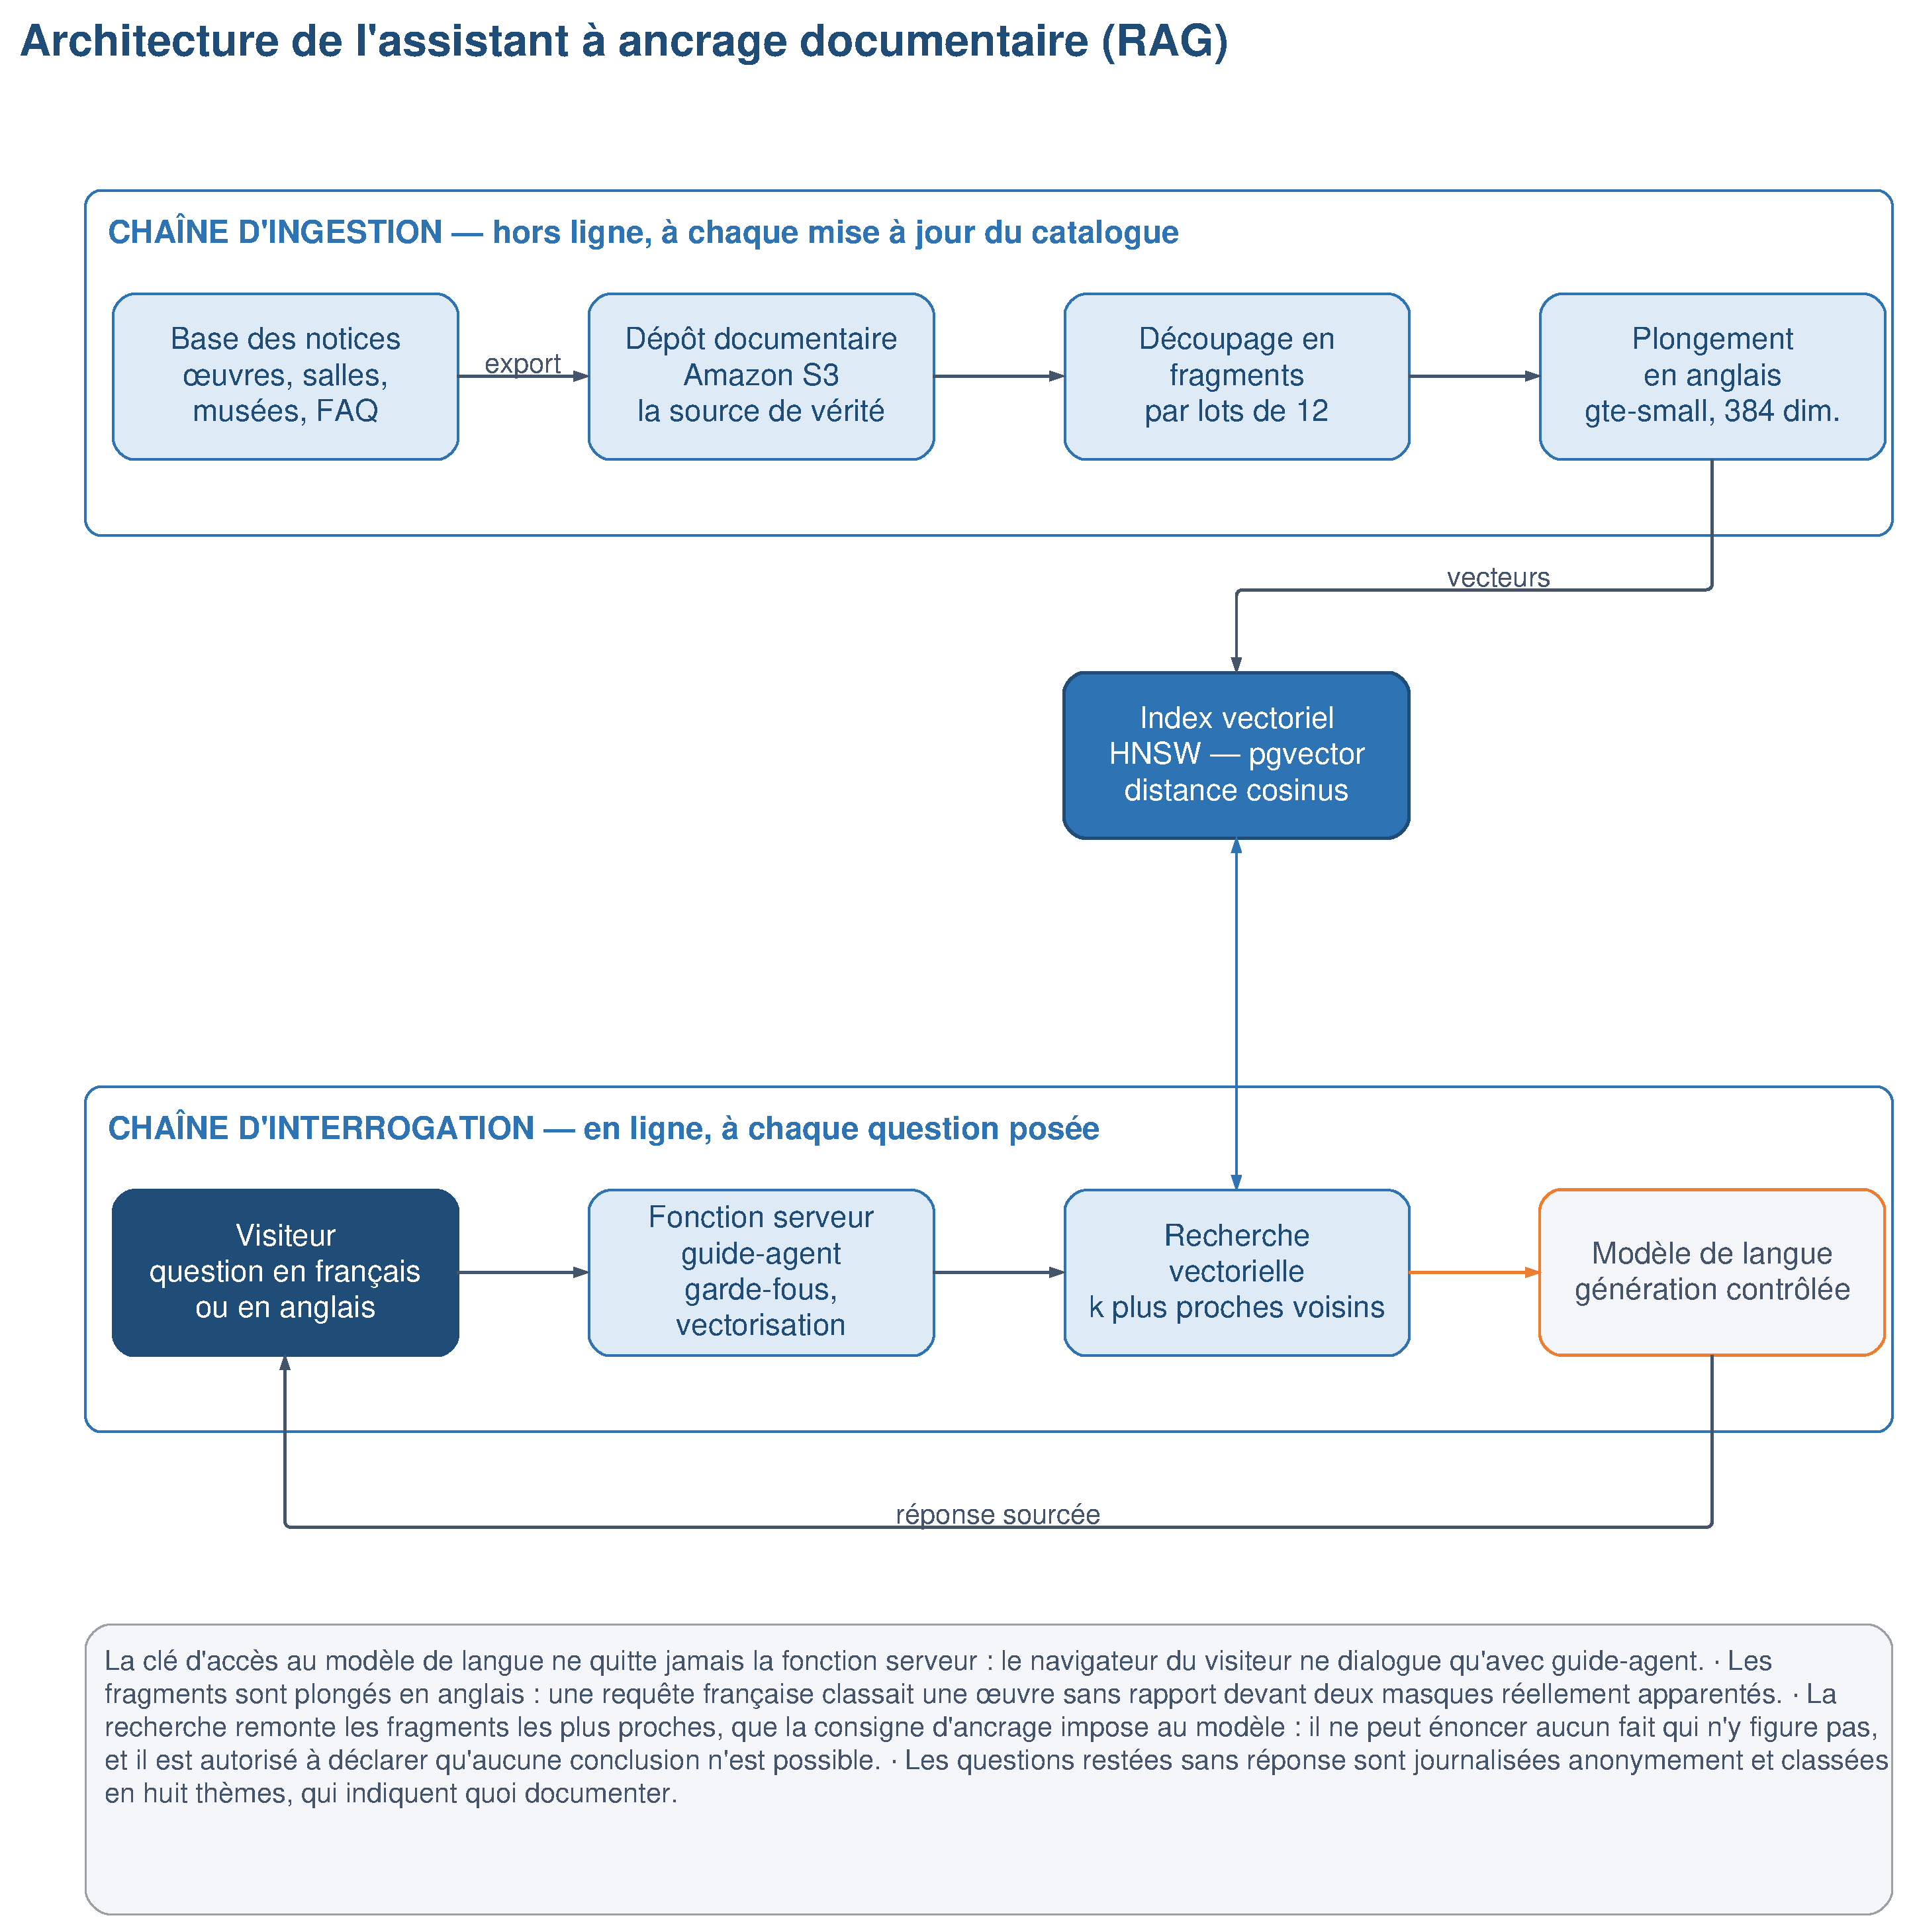
\includegraphics[width=\textwidth]{figures/rag-musea.pdf}
\caption{Architecture de l'assistant conversationnel à ancrage documentaire (RAG)}
\label{fig:rag}
\source{Élaboré par nos soins.}
\end{figure}

\subsubsection{Le moteur de visite immersive}

L'impossibilité d'ajouter des bibliothèques a conduit à écrire le moteur de
panorama de bout en bout. Il restitue la salle sans aucun maillage, ce qui
supprime les défauts de facettes, et efface la couture verticale visible à la
jonction des bords de l'image. Les points d'intérêt ne sont pas dessinés dans
l'image : ce sont de véritables boutons superposés au rendu, ce qui les laisse
atteignables au clavier et restituables par un lecteur d'écran.

\subsubsection{Chaîne de numérisation tridimensionnelle et réalité augmentée}

Il faut distinguer deux usages de la trois dimensions, car ils ne portent pas
sur les mêmes sujets et n'appellent pas les mêmes traitements.

\textbf{Les œuvres} sont numérisées par \textbf{photogrammétrie} : trois orbites
de prises de vue guidées autour de la pièce, puis reconstruction sur une
instance à processeur graphique. Le modèle obtenu est destiné à la consultation
à l'écran, où le visiteur le fait pivoter et l'examine sous tous ses angles.

\textbf{Les habitations et les espaces à visiter} relèvent au contraire de la
\textbf{réalité augmentée}. Ils sont relevés au moyen du \textbf{capteur LiDAR}
d'un téléphone, qui mesure directement les distances et fournit en quelques
minutes une géométrie correctement dimensionnée, puis exportés dans les deux
formats du web immersif, \textbf{GLB} pour les appareils Android et
\textbf{USDZ} pour ceux d'Apple. Le visiteur peut alors faire apparaître
l'espace dans son propre environnement, à l'échelle, au moyen des visionneuses
intégrées aux systèmes mobiles : \emph{AR Quick Look} sur iOS, et le composant
\texttt{model-viewer} associé à \emph{Scene Viewer} sur Android. Aucune
application n'a donc à être installée, ce qui était la condition posée par le
public visé.

Cette dualité de formats n'est pas un détail : produire un seul des deux revient
à priver de la fonction la moitié des visiteurs. Le système enregistre pour
chaque espace le modèle GLB, le modèle USDZ et le facteur d'échelle appliqué à
l'export, faute de quoi un relevé exprimé en centimètres arriverait cent fois
trop grand dans la scène réelle. La restitution se fait aux dimensions relevées
et non à une taille choisie par le visiteur, car l'intérêt du procédé est
précisément de faire éprouver l'échelle véritable du lieu.

Enfin, la réalité augmentée supposant un téléphone alors qu'une présentation se
tient devant un ordinateur, un encodeur de codes QR a été écrit afin que le
public puisse scanner l'écran et poursuivre sur son propre appareil.

\subsubsection{Infrastructure d'hébergement}

L'application étant un site statique, l'infrastructure retenue est délibérément
minimale : un espace de stockage privé, chiffré et versionné, servi par un
réseau de diffusion mondial au moyen d'un contrôle d'accès à l'origine ; un
certificat de sécurité couvrant le domaine principal et l'ensemble de ses
sous-domaines ; et des enregistrements de noms de domaine dotés d'un caractère
générique, qui font exister l'adresse de chaque organisation sans qu'il soit
nécessaire de créer un enregistrement par institution.

Deux réglages conditionnent le bon fonctionnement du dispositif : le
\textbf{repli applicatif}, qui renvoie la page d'accueil lorsqu'une adresse
profonde est demandée, faute de quoi les codes QR de réalité augmentée
échoueraient, et les \textbf{durées de cache différenciées} selon la famille de
fichiers, sans quoi le site resterait figé sur une version périmée.

La figure~\ref{fig:cloud} restitue l'ensemble de cette
infrastructure telle
qu'elle est décrite dans le code Terraform du projet. Elle se lit sur deux
plans, que la teinte des tuiles distingue.

\begin{figure}[!ht]
\centering
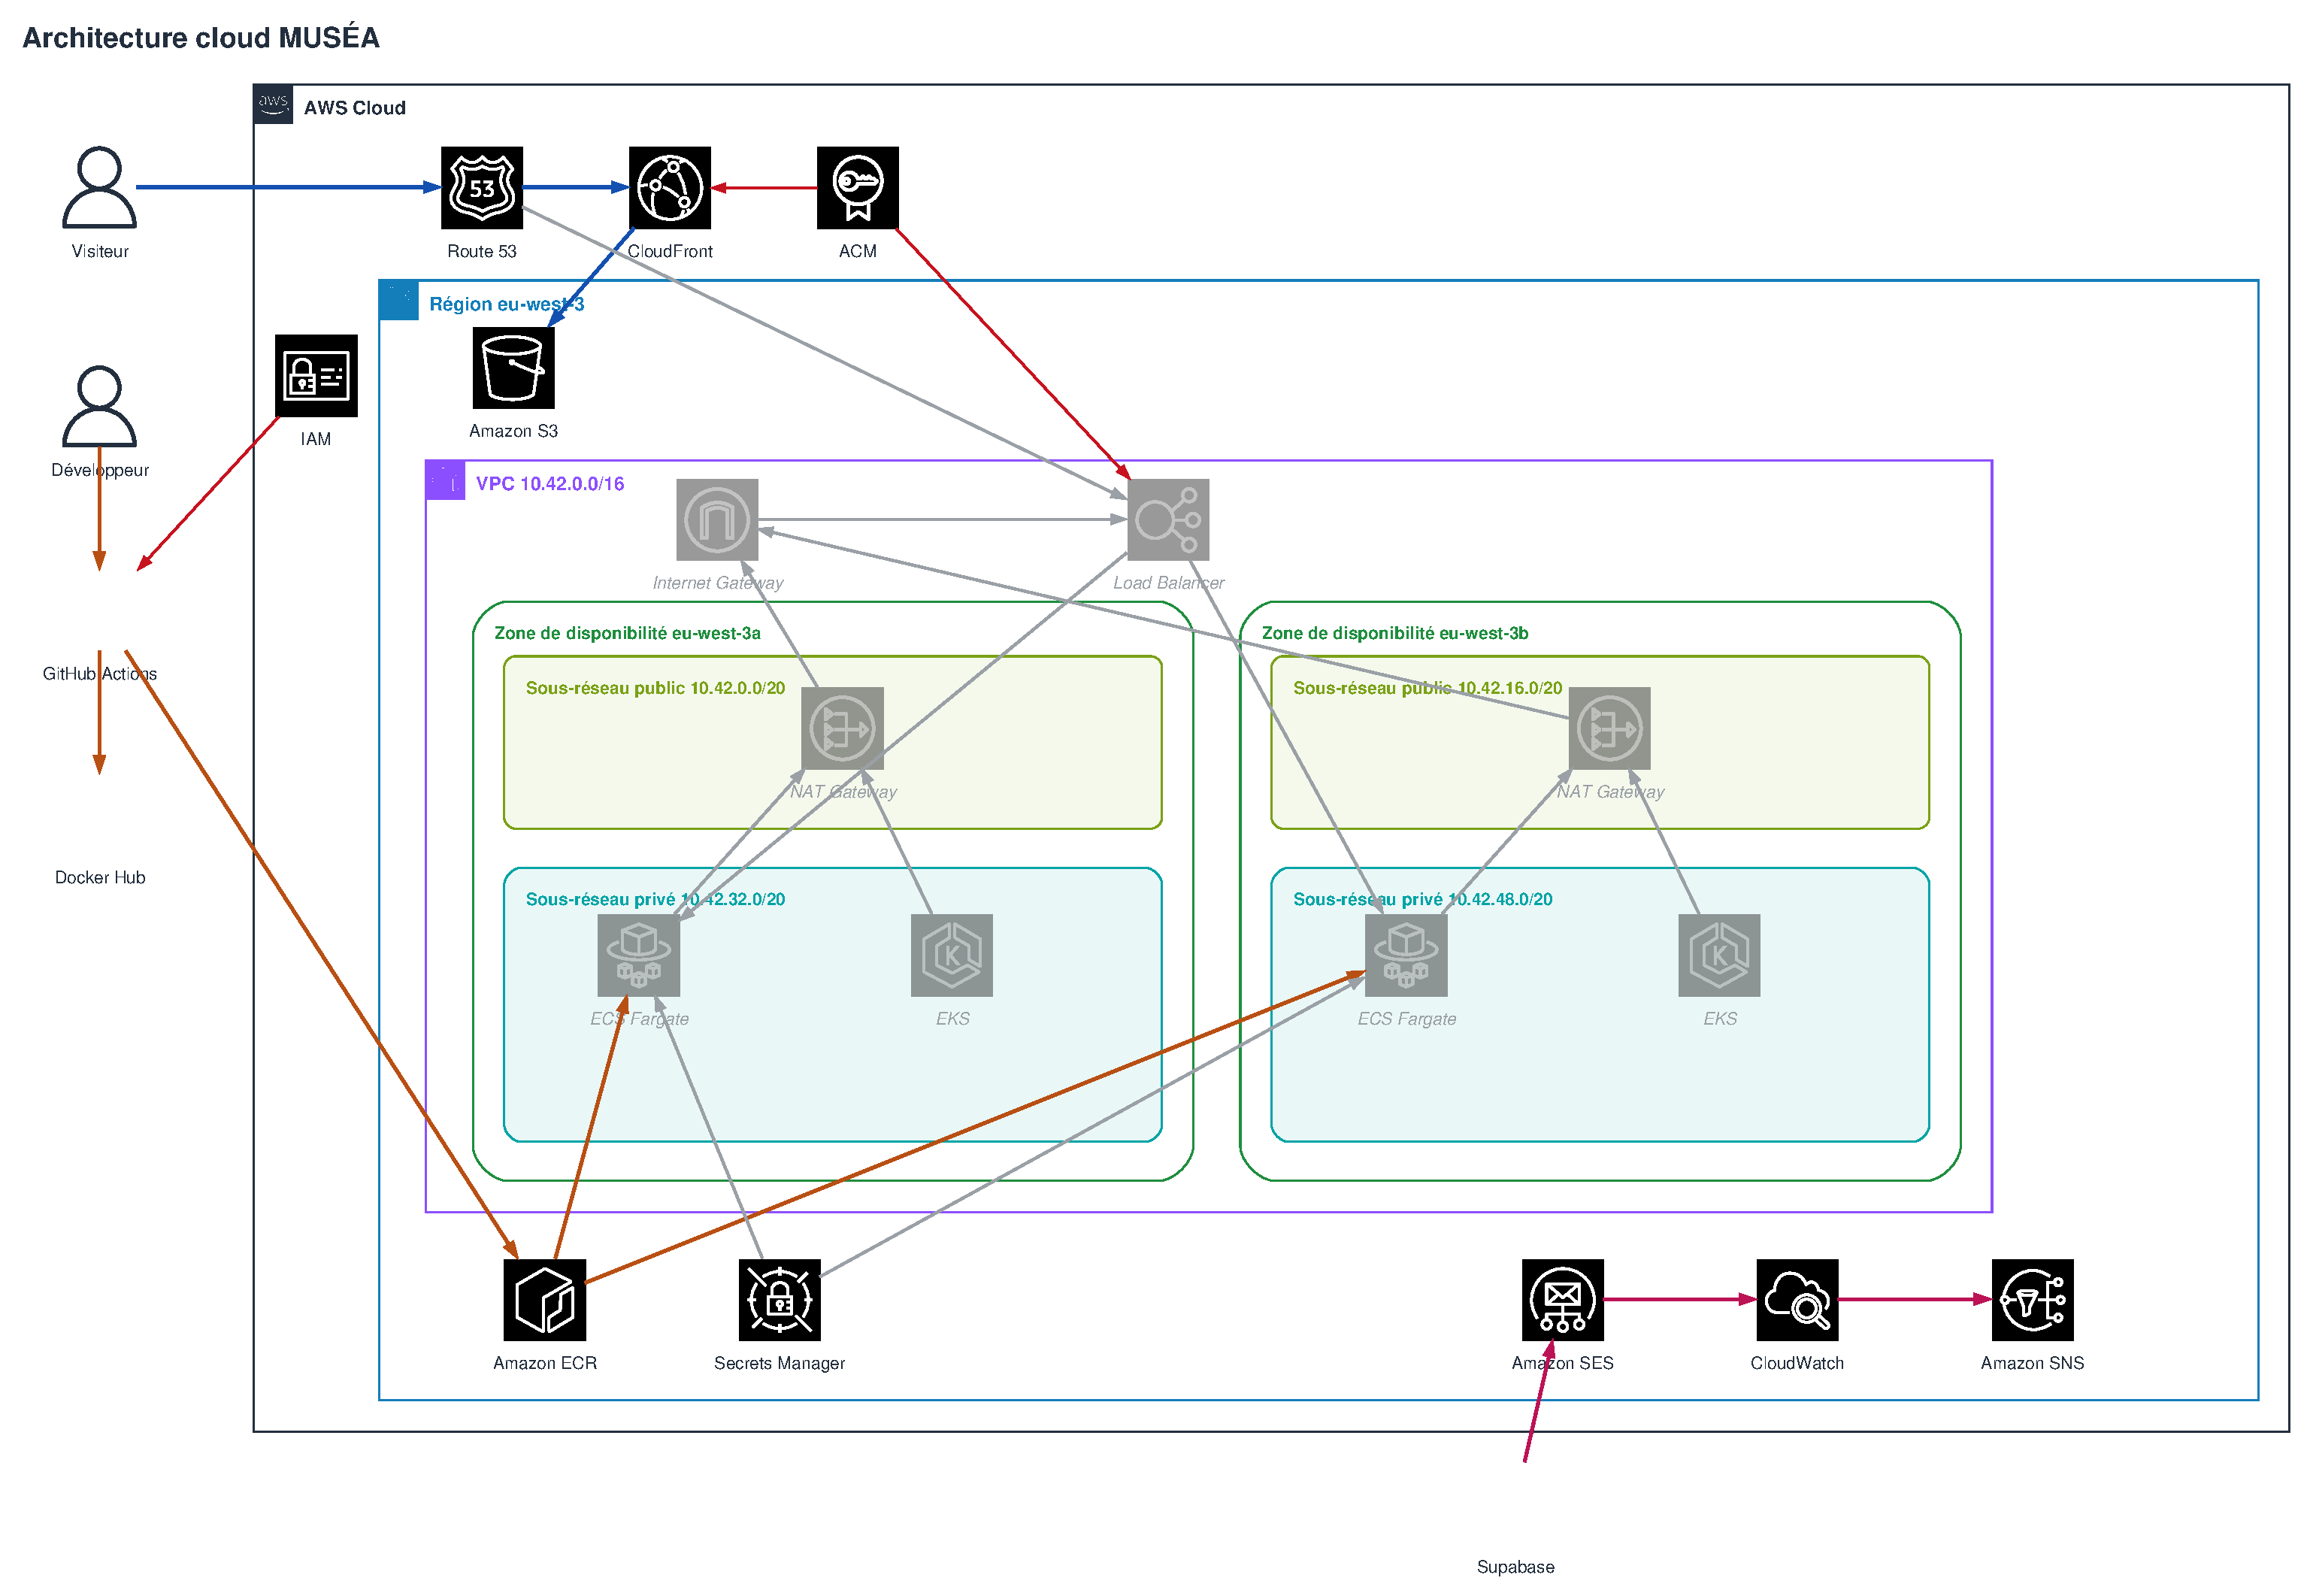
\includegraphics[width=\textwidth]{figures/architecture-cloud-musea.pdf}
\caption{Architecture de l'infrastructure d'hébergement en nuage}
\label{fig:cloud}
\source{Élaboré par nos soins d'après la description Terraform du projet.}
\end{figure}

\textbf{Ce qui est en service} figure en pleine couleur, et l'on y suit deux
chemins. Le premier est celui d'une requête de visiteur : le navigateur
interroge \emph{Route 53}, qui résout aussi bien le domaine principal que le
sous-domaine de chaque institution ; \emph{CloudFront} sert alors le contenu,
sous le certificat délivré par \emph{ACM}, et il est le seul à pouvoir lire le
compartiment \emph{Amazon S3}. Le second est celui de la livraison : le
développeur dépose sa modification, \emph{GitHub Actions} construit l'image et
la dépose sur \emph{Docker Hub} et sur \emph{Amazon ECR}, en se présentant à
\emph{IAM} avec un jeton de courte durée plutôt qu'avec une clé permanente. À
ces deux chemins s'ajoutent les services de support : \emph{Secrets Manager}
pour les secrets, \emph{SES} pour les envois de courrier, \emph{CloudWatch} et
\emph{SNS} pour la surveillance et l'alerte. Hors du nuage AWS, \emph{Supabase}
porte la base de données, l'authentification et les fonctions serveur.

\textbf{Ce qui est décrit mais non appliqué} figure en grisé : le réseau privé
virtuel et ses deux zones de disponibilité, la passerelle Internet, le
répartiteur de charge, les passerelles de traduction d'adresses et les
exécutions conteneurisées \emph{ECS Fargate} et \emph{EKS}. Ces ressources
constituent très exactement l'écart entre les 29 ressources décrites dans le
code et les 19 réellement créées à la mise en ligne : elles sont écrites,
validées, mais délibérément non appliquées, parce qu'un site statique n'en a pas
besoin et qu'elles coûteraient sans rien servir. Elles sont l'objet de
l'intervention proposée au chapitre~\ref{chap:diagnostic}. Ce schéma dit donc
deux choses à la fois : l'état déployé, et la trajectoire déjà écrite.


\subsubsection{La chaîne d'intégration et de déploiement continus}

La chaîne mise en place comporte deux enchaînements, mis en regard à la
figure~\ref{fig:devops-actuel}. Le premier, déclenché à
chaque dépôt de modification, compile l'application et exécute une série de
contrôles sur le résultat produit, présence des fichiers attendus, validité des
modèles tridimensionnels, présence de l'adresse du service de données dans le
paquet compilé ; ce dernier contrôle mérite un mot, car sans cette adresse le
site s'affiche parfaitement et ne charge aucune donnée, la panne la plus
déroutante qui soit. Cet enchaînement s'arrête net, sans rien publier, dès qu'un
contrôle échoue.

\begin{figure}[!ht]
\centering
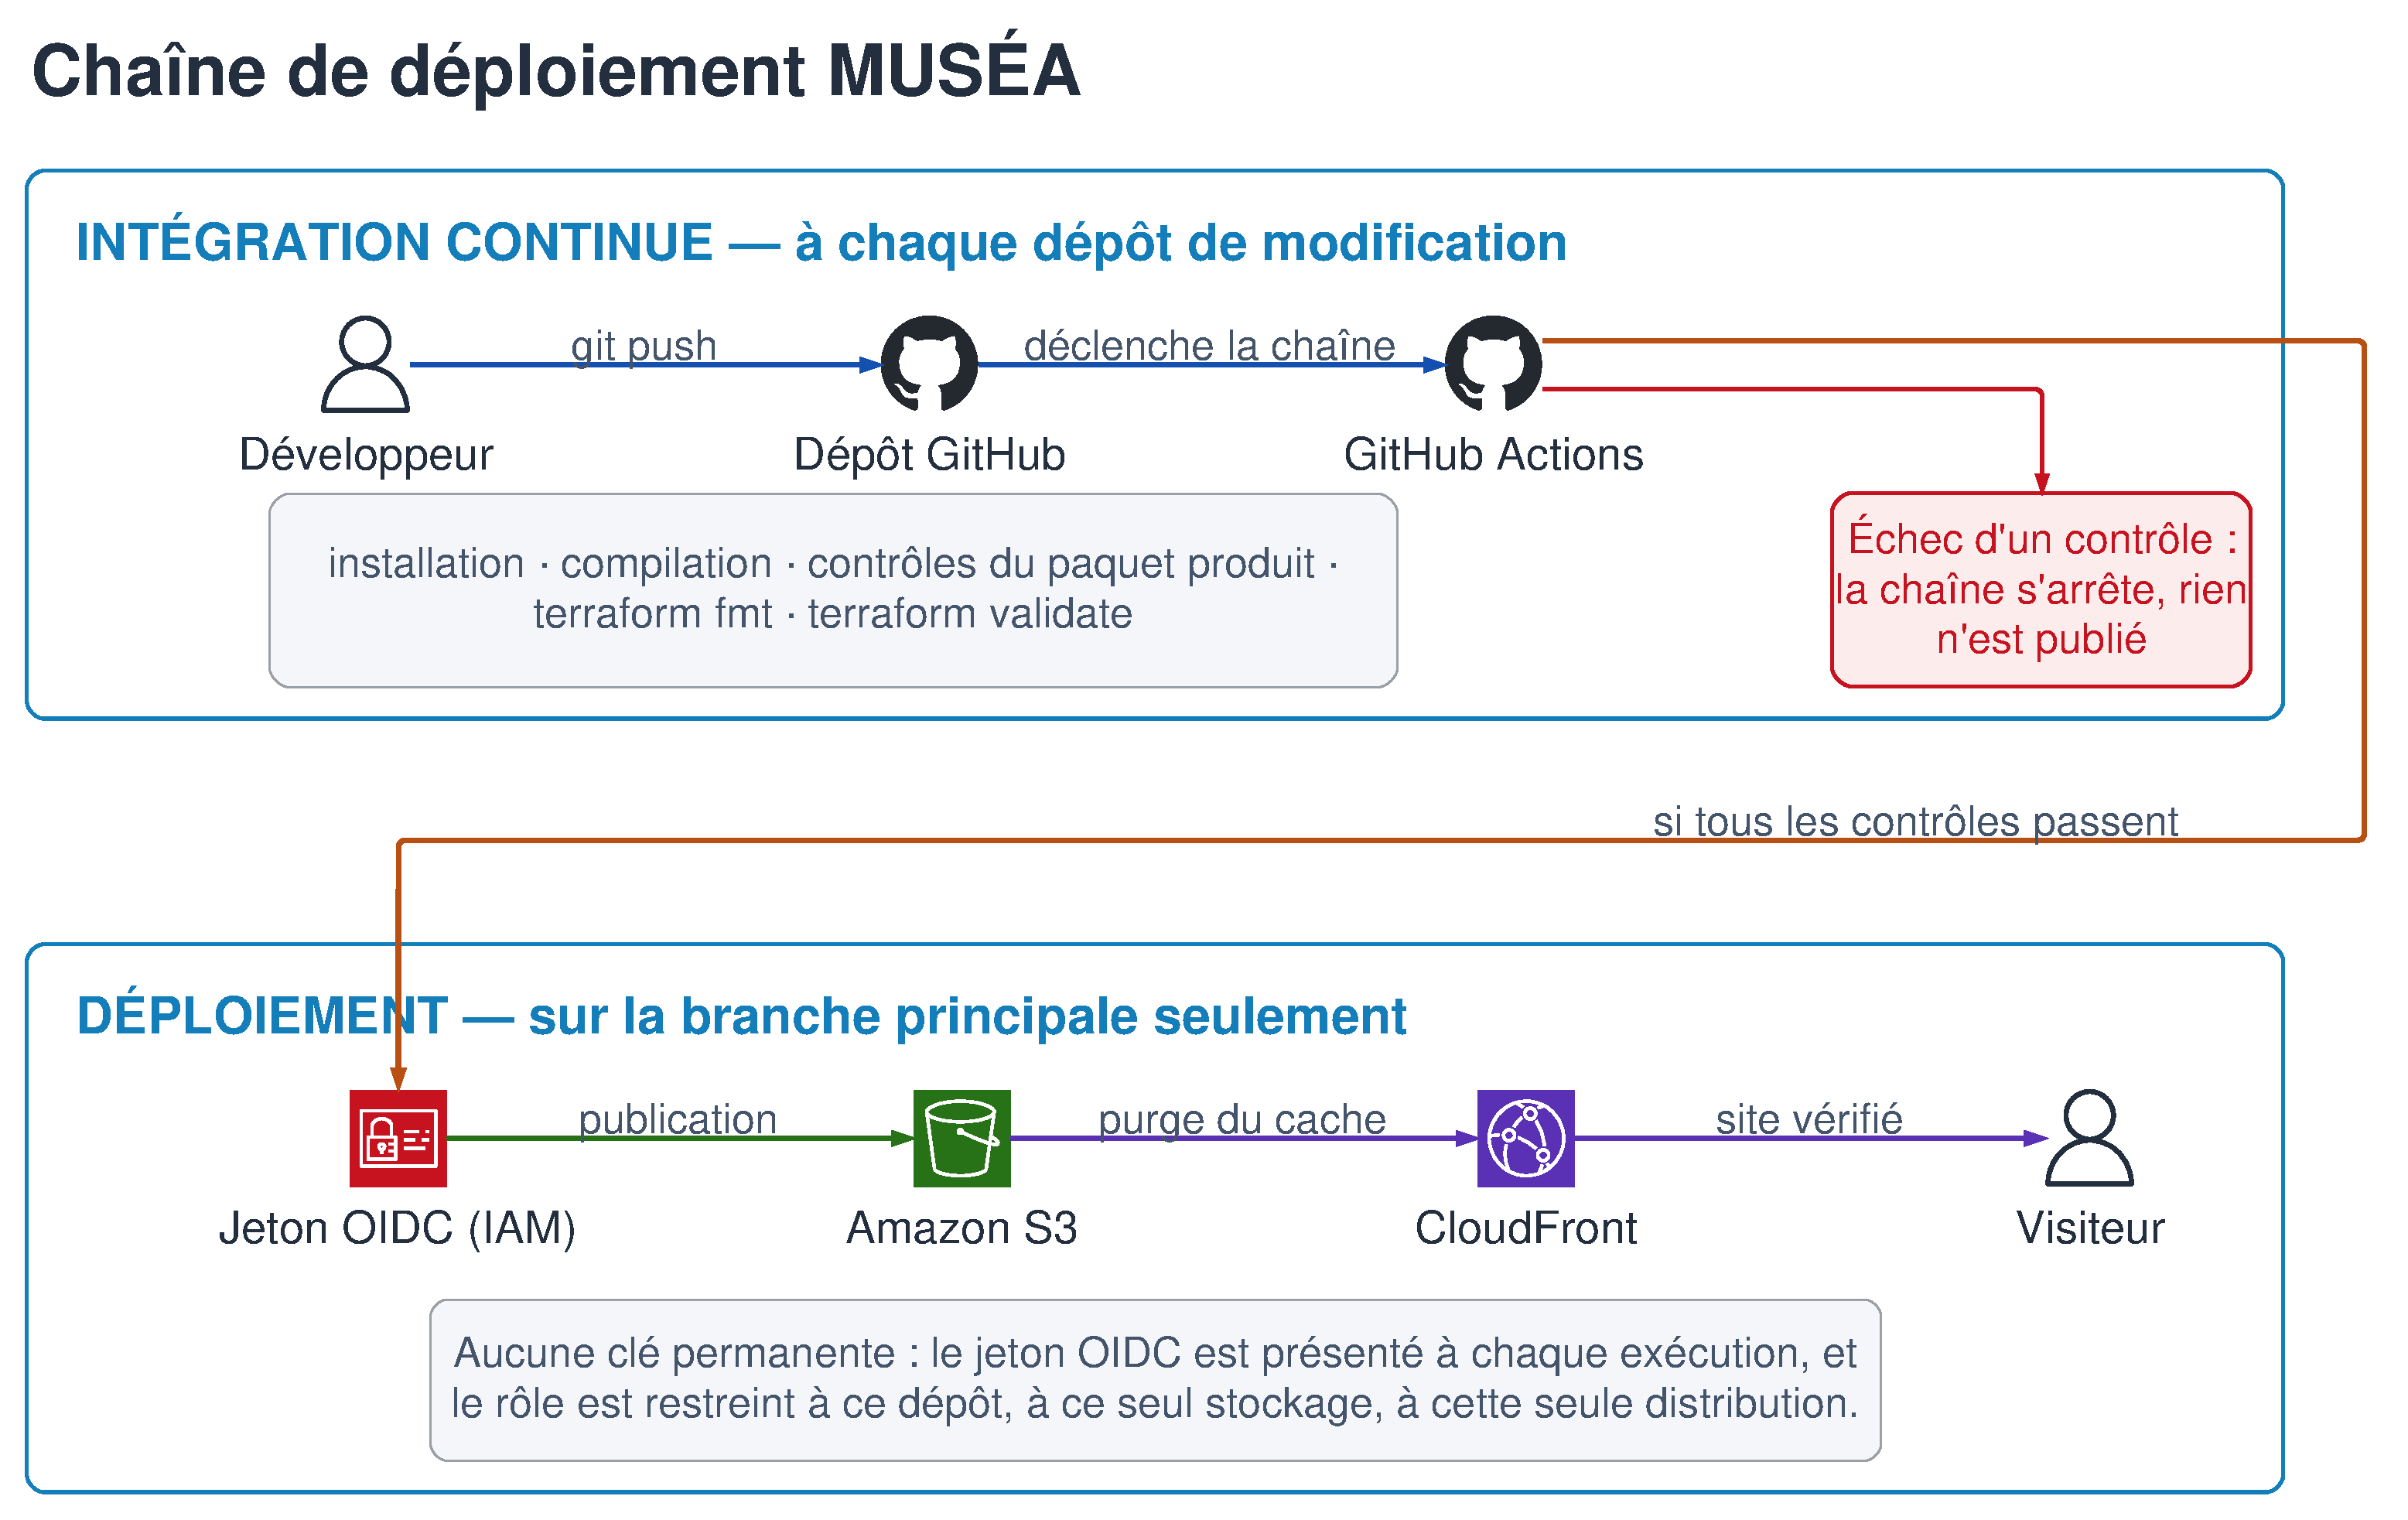
\includegraphics[width=\textwidth]{figures/deploiement-musea.pdf}
\caption{Chaîne d'intégration et de déploiement continus en service}
\label{fig:devops-actuel}
\source{Élaboré par nos soins d'après les fichiers de description des chaînes du projet.}
\end{figure}

Le second n'est atteint que si tous les contrôles passent, et seulement depuis
la branche principale. Il publie l'application, purge le cache de diffusion,
puis, point essentiel, \textbf{vérifie le site en ligne} : on ne contrôle pas ce
que l'on croit avoir déployé, on contrôle ce que le visiteur reçoit. C'est cette
dernière vérification qui distingue la chaîne d'une simple automatisation de
copie. L'authentification auprès du fournisseur de nuage ne repose enfin sur
aucune clé permanente : un jeton de courte durée est présenté à chaque
exécution, et le rôle correspondant est restreint au dépôt de code concerné, à
ce seul espace de stockage et à cette seule distribution.


% =============================================================================
\subsubsection{Ressources mobilisées et coût du projet}

\paragraph{Ressources matérielles, logicielles et de service.} Le détail des
moyens mobilisés figure aux tableaux~\ref{tab:materiel}
et~\ref{tab:logiciel}.

\begin{table}[!ht]
\centering
\caption{Ressources matérielles mobilisées}
\label{tab:materiel}
\small
\begin{tabularx}{\textwidth}{|L{3.2cm}|X|C{1.3cm}|R{2.0cm}|R{2.0cm}|}
\hline
\rowcolor{keycetete}
\thead{Matériel} & \thead{Caractéristiques} & \thead{Qté} & \thead{P.U. (FCFA)} & \thead{Total (FCFA)} \\ \hline
Ordinateur portable & Processeur 8 cœurs, 32 Go de mémoire vive, 1 To de disque à semi-conducteurs & 1 & 450 000 & 450 000 \\ \hline
Écran secondaire & 24 pouces, 1920 $\times$ 1080 & 1 & 100 000 & 100 000 \\ \hline
Téléphone à capteur LiDAR & iPhone 15 Pro, acquisition tridimensionnelle et essais de réalité augmentée & 1 & 400 000 & 400 000 \\ \hline
Disque externe & 1 To, à semi-conducteurs, sauvegarde des prises de vue et des maillages & 1 & 55 000 & 55 000 \\ \hline
Onduleur & 650 VA, protection contre les coupures de courant & 1 & 48 000 & 48 000 \\ \hline
Éclairage d'appoint & 2 panneaux à diodes, prises de vue des œuvres & 1 & 45 000 & 45 000 \\ \hline
Trépied et tête panoramique & Prises de vue à 360 degrés & 1 & 35 000 & 35 000 \\ \hline
\rowcolor{keycetotal}
\multicolumn{4}{|l|}{\textbf{Coût total des ressources matérielles}} & \textbf{1 133 000} \\ \hline
\end{tabularx}
\source{Relevé des prix pratiqués à Bafoussam et à Douala, juin 2026.}
\end{table}

\begin{table}[!ht]
\centering
\caption{Ressources logicielles et services mobilisés}
\label{tab:logiciel}
\small
\begin{tabularx}{\textwidth}{|L{4.4cm}|X|R{2.4cm}|}
\hline
\rowcolor{keycetete}
\thead{Logiciel ou service} & \thead{Rôle} & \thead{Coût (FCFA)} \\ \hline
Windows 11 Professionnel & Système d'exploitation du poste de développement & 90 350 \\ \hline
Connexion Internet & Forfait données, deux mois & 60 000 \\ \hline
Nom de domaine \texttt{.store} & Adresse publique de la plateforme, un an & 9 000 \\ \hline
Hébergement et diffusion AWS & Stockage, réseau de diffusion, noms de domaine et certificats, deux mois & 1 460 \\ \hline
Calcul graphique ponctuel & Instance à processeur graphique pour la photogrammétrie, 6 heures & 1 900 \\ \hline
Supabase & Base de données, authentification et fonctions serveur, palier gratuit & 0 \\ \hline
Groq & Génération de texte, palier gratuit & 0 \\ \hline
ElevenLabs & Synthèse vocale, palier de découverte & 0 \\ \hline
Visual Studio Code, Git, Docker, Terraform & Développement et industrialisation, logiciels libres & 0 \\ \hline
Meshroom, Blender & Photogrammétrie et préparation des maillages, logiciels libres & 0 \\ \hline
\rowcolor{keycetotal}
\multicolumn{2}{|l|}{\textbf{Coût total des ressources logicielles et services}} & \textbf{162 710} \\ \hline
\end{tabularx}
\source{Factures et relevés de consommation, juin--août 2026.}
\end{table}

Ces deux relevés appellent une lecture. Le matériel, d'un montant de
1~133~000~FCFA, est constitué à 91~\% d'un poste de travail réutilisable : il
s'agit d'un investissement acquis une fois pour toutes, et non d'une dépense
propre au projet. Les logiciels et services, d'un montant de 162~710~FCFA,
tiennent à 92~\% au système d'exploitation et à la suite bureautique,
c'est-à-dire à des postes qui existeraient de toute façon ; la chaîne technique
proprement dite, base de données, génération de texte, synthèse vocale,
développement et industrialisation, n'a rien coûté.

\paragraph{Coût de l'infrastructure en nuage.}

Le coût de l'infrastructure ne se devine pas, il se relève. Conformément aux
principes exposés au chapitre~1, la dépense a été estimée au moyen
d'\textbf{Infracost}, un outil libre qui lit les fichiers Terraform décrivant
l'infrastructure, identifie chacune des ressources qu'ils déclarent, interroge
le barème public du fournisseur et en déduit le coût mensuel correspondant.

\textbf{Pourquoi cet outil plutôt qu'un relevé de facturation.} Trois raisons
ont commandé ce choix, et elles tiennent toutes à la question posée par la
Fondation lors des entretiens : \emph{combien cela coûtera-t-il une fois le
stagiaire parti ?}

D'abord, \textbf{le moment de la mesure}. Une console de facturation constate
une dépense déjà engagée : elle apprend en fin de mois ce que l'on a consommé.
Infracost, lui, chiffre la modification \emph{avant} qu'elle ne soit appliquée,
c'est-à-dire au moment où l'on peut encore y renoncer. Ajouter une passerelle
NAT ou un répartiteur de charge dans un fichier Terraform paraît anodin ; savoir
que ce geste engage plusieurs dizaines de dollars par mois change la décision,
et ce savoir doit intervenir avant la fusion du code, non après.

Ensuite, \textbf{la reproductibilité}. Le relevé de facturation dépend du compte
sur lequel il est établi et ne se transmet pas. L'estimation d'Infracost, elle,
se déduit des seuls fichiers versionnés : n'importe qui, muni du dépôt, obtient
le même chiffre. C'est ce qui rend le coût annoncé dans ce rapport vérifiable
par un tiers, ce qu'un relevé de compte privé ne permettrait pas.

Enfin, \textbf{l'inscription dans la chaîne d'intégration continue}. L'outil
s'exécute automatiquement à chaque proposition de modification de
l'infrastructure et en publie l'écart de coût. La maîtrise de la dépense cesse
alors d'être un audit ponctuel pour devenir un contrôle permanent, ce qui
correspond exactement au troisième temps de la démarche FinOps exposée au
chapitre~1, \emph{opérer}.

\textbf{Ce que l'outil ne dit pas.} Une réserve doit être posée, faute de quoi
le chiffre serait mal lu. Infracost évalue le coût \emph{structurel} des
ressources déclarées, celui qui existe indépendamment de l'usage : une zone
hébergée, un certificat, un serveur allumé. Il ne peut pas deviner les postes
proportionnels à la consommation, volume stocké et données transférées, qu'il
laisse à zéro sauf à lui fournir un fichier d'hypothèses d'usage. Les montants
du tableau~\ref{tab:finops} combinent donc les deux sources : l'estimation
structurelle pour les ressources déclarées, la consommation constatée pour les
postes variables. Le tableau détaille la dépense par service.

\begin{table}[!ht]
\centering
\caption{Détail du coût de l'infrastructure en nuage (relevé FinOps)}
\label{tab:finops}
\small
\begin{tabularx}{\textwidth}{|L{3.8cm}|X|R{2.2cm}|R{2.2cm}|}
\hline
\rowcolor{keycetete}
\thead{Service} & \thead{Usage} & \thead{Coût mensuel (FCFA)} & \thead{Sur 2 mois (FCFA)} \\ \hline
Route 53 & Zone hébergée du domaine et enregistrements joker & 310 & 620 \\ \hline
Amazon S3 & Stockage du site, des modèles 3D et des médias & 90 & 180 \\ \hline
CloudFront & Réseau de diffusion et certificat de sécurité & 330 & 660 \\ \hline
Certificate Manager & Certificats de sécurité, service gratuit & 0 & 0 \\ \hline
\rowcolor{keycetotal}
\multicolumn{2}{|l|}{\textbf{Total hébergement récurrent}} & \textbf{730} & \textbf{1 460} \\ \hline
EC2 (processeur graphique) & Reconstruction photogrammétrique, 6 heures, instance arrêtée hors usage & — & 1 900 \\ \hline
\rowcolor{keycetotal}
\multicolumn{3}{|l|}{\textbf{Total infrastructure sur la période du stage}} & \textbf{3 360} \\ \hline
\end{tabularx}
\source{Estimation \emph{Infracost} établie sur les fichiers de description de
l'infrastructure, période du 20 juin au 20 août 2026.}
\end{table}

Ce relevé appelle un commentaire qui dépasse la simple comptabilité. Le coût
récurrent de l'hébergement s'établit à environ \textbf{730 FCFA par mois}, soit
moins de 9 000 FCFA par an. Ce montant, dérisoire au regard du budget d'une
institution, tient à un choix d'architecture : l'application étant un site
statique servi par un réseau de diffusion, elle ne mobilise aucun serveur en
fonctionnement permanent. Le seul poste réellement coûteux, le calcul graphique
nécessaire à la photogrammétrie, est ponctuel et l'instance correspondante
s'arrête automatiquement lorsqu'elle n'est pas sollicitée. C'est là l'apport
concret de la démarche FinOps : non pas économiser après coup, mais concevoir de
telle sorte que la dépense reste proportionnée à l'usage réel.

\paragraph{Coût total du projet.}

\begin{table}[!ht]
\centering
\caption{Coût total du projet}
\label{tab:couttotal}
\small
\begin{tabularx}{\textwidth}{|X|R{3.4cm}|}
\hline
\rowcolor{keycetete}
\thead{Libellé} & \thead{Montant (FCFA)} \\ \hline
Ressources matérielles & 1 133 000 \\ \hline
Ressources logicielles et services & 162 710 \\ \hline
Sous-total & 1 295 710 \\ \hline
Marge d'erreur (3 \%) & 38 871 \\ \hline
\rowcolor{keycetotal}
\textbf{Coût total du projet} & \textbf{1 334 581} \\ \hline
\end{tabularx}
\source{Élaboré par nos soins à partir des tableaux~\ref{tab:materiel}
et~\ref{tab:logiciel}.}
\end{table}

Le tableau~\ref{tab:couttotal} montre que 85 \% du coût total est constitué de
matériel réutilisable, acquis une fois pour toutes. La reconduction du
dispositif dans une autre institution ne suppose donc pas de reproduire cette
dépense : elle n'appelle que le coût récurrent d'hébergement relevé au
tableau~\ref{tab:finops}.

\subsection{Les résultats obtenus}
\label{sec:resultats}

Le dispositif livré compte une vingtaine de fonctionnalités. Les décrire toutes
n'aurait pas d'intérêt : cette section retient celles qui portent les hypothèses
de l'étude, et renvoie pour les autres au tableau~\ref{tab:mesures}, qui en
donne les valeurs mesurées.

\subsubsection{La gestion des collections et le site public}

Le back-office permet d'enregistrer les musées, puis les salles qui les
composent, puis les œuvres qu'abritent ces salles, chaque œuvre portant un nom,
une description, une histoire, des médias, une grille tarifaire et, le cas
échéant, ses modèles tridimensionnels. Cette fonctionnalité est le socle de tout
le reste : sans inventaire structuré, ni la visite immersive, ni l'assistant, ni
le rapprochement documentaire ne disposent de matière.

\begin{figure}[!ht]
\centering
\capture{cap-01-erp-musees.png}
\caption{Back-office : la gestion des musées de l'institution}
\label{fig:cap-erp}
\source{Capture d'écran de la plateforme MUSÉA, septembre 2026.}
\end{figure}

La figure~\ref{fig:cap-erp} montre l'écran de gestion des musées. Trois éléments
méritent d'être relevés : l'interrupteur \emph{En ligne / Hors ligne} porté par
chaque fiche, qui fait de la publication une décision explicite du personnel, le
musée marqué \emph{Brouillon} restant invisible du public ; les boutons
\emph{Exporter le modèle Excel} et \emph{Importer}, qui répondent à l'objection
formulée en entretien d'avoir à ressaisir un inventaire déjà tenu sur tableur ;
et l'organisation en fiches illustrées plutôt qu'en tableau de base de données,
le vocabulaire affiché étant celui du métier et non celui du modèle relationnel.

Chaque institution dispose par ailleurs d'un site public présentant son
identité, ses musées, son catalogue et sa boutique. L'ensemble des éléments
visibles, marque, couleurs, images d'accueil, textes des pages de connexion, est
modifiable depuis le back-office : aucun texte n'est figé dans le code, de sorte
qu'une institution qui change de charte graphique n'a pas besoin d'un
développeur.

\begin{figure}[!ht]
\centering
\capture{cap-02-site-public.png}
\caption{Site public : l'en-tête de l'institution et la section des œuvres modélisées}
\label{fig:cap-public}
\source{Capture d'écran de la plateforme MUSÉA, septembre 2026.}
\end{figure}

La figure~\ref{fig:cap-public} donne à voir ce que rencontre le visiteur : une
navigation réduite à trois entrées, \emph{Musées}, \emph{Nos boutiques} et
\emph{Généalogie}, qui sont les trois fils du projet, et la section « Tournez
autour de l'œuvre » où chaque pièce effectivement modélisée porte la pastille
\emph{3D}. Le bouton \emph{Back-office} placé dans l'en-tête mérite d'être
relevé : le site public et l'outil de gestion ne sont pas deux applications
séparées, et un membre du personnel déjà connecté passe de l'un à l'autre sans
changer d'adresse.

\subsubsection{La restitution spatiale : visite à 360 degrés, 3D et réalité augmentée}

La restitution repose sur trois dispositifs distincts, qui ne répondent pas à la
même question. \textbf{Le parcours à 360 degrés} répond à « où suis-je ? » : le
visiteur entre dans une salle, pivote librement, passe à la salle suivante par
un point de passage et touche un objet pour en ouvrir la fiche. \textbf{Le
modèle tridimensionnel d'une œuvre} répond à « à quoi ressemble-t-elle sous tous
ses angles ? » : depuis la fiche, la pièce se fait pivoter à l'écran.

\textbf{La réalité augmentée}, enfin, répond à « quelle taille cela fait-il, et
comment est-ce chez moi ? », et elle ne porte pas sur les œuvres mais sur
\textbf{les habitations et les espaces à visiter}. Relevés au capteur LiDAR puis
exportés en GLB et en USDZ, ces espaces se posent dans l'environnement réel du
visiteur, à l'échelle, au moyen des visionneuses intégrées aux téléphones, sans
installation d'application. C'est là que se joue le « retour au pays » : faire
apparaître, dans le salon d'un membre de la diaspora, une case de Bangoulap à sa
dimension véritable. Sur ordinateur, où la réalité augmentée n'a pas de sens, un
code QR renvoie le visiteur vers son téléphone.

Un mode de démonstration dessine enfin une salle stylisée au vol, ce qui a rendu
le parcours démontrable \emph{avant} les prises de vue réelles.

\subsubsection{Le guide vocal en temps réel et l'assistant à ancrage documentaire}

C'est la fonctionnalité la plus démonstrative du dispositif. \textbf{Pendant que
le visiteur fait tourner un objet en trois dimensions, il peut parler à l'œuvre
et celle-ci lui répond de vive voix}, sans passer par le clavier. La chaîne est
entièrement temps réel : la voix du visiteur est transmise à un service
conversationnel vocal, transcrite, portée à l'assistant documentaire, et la
réponse est restituée en synthèse vocale pendant que la manipulation du modèle
se poursuit. L'objet cesse ainsi d'être une pièce que l'on regarde pour devenir
un interlocuteur, ce qui est très exactement l'objet d'une médiation muséale :
la médiation est d'abord orale, et l'écoute libère le regard, puisqu'on ne peut
pas lire une notice et observer une œuvre en même temps.

La fiabilité de cette parole repose sur l'\textbf{ancrage documentaire}, ou
génération augmentée par la recherche. Le principe tient en trois temps. Les
documents de l'institution sont d'abord découpés en fragments, chacun converti
en un vecteur numérique qui en résume le sens ; la question du visiteur est
ensuite convertie de la même manière, ce qui permet de retrouver les fragments
les plus proches, non par mots-clés mais par proximité de sens ; ces fragments
sont enfin remis au modèle de langue avec la consigne de ne répondre qu'à partir
d'eux. Le modèle ne puise donc pas dans ce qu'il a appris ailleurs : il
reformule ce que l'institution a écrit, et cite ses sources.

Quatre garde-fous complètent le dispositif : un refus poli des sujets hors
périmètre, prononcé sans même solliciter le modèle de langue ; une réponse
chaleureuse aux salutations ; une restriction de la recherche au musée ou à la
salle où se trouve le visiteur ; et une consigne interdisant d'énoncer un fait
absent des documents fournis, assortie de l'autorisation explicite de déclarer
son ignorance. Les questions restées sans réponse sont enfin consignées de
manière anonyme et classées en huit thèmes, puis présentées au personnel sous
forme de conseils : au lieu de constater un échec, le journal indique quoi
documenter.

\subsubsection{La mémoire réunifiée et la généalogie}

À partir de la notice d'une œuvre, le système interroge en parallèle cinq
collections ouvertes, ordonne les résultats par proximité de sens, fait
justifier les rapprochements les plus probables, puis les soumet au conservateur
qui valide, écarte ou corrige. Les correspondances validées apparaissent sur la
fiche publique avec le nom du musée détenteur et le numéro d'inventaire. Une
mesure comparative établit le résultat le plus instructif de l'étude : une
recherche formulée en français ramène 16 résultats dont le meilleur atteint 57
sur 100, tandis que la même recherche reformulée dans le vocabulaire de
catalogage anglais n'en ramène que 5, mais dont le meilleur atteint 85. Ce
résultat est interprété au chapitre~\ref{chap:diagnostic}.

Un arbre généalogique bidirectionnel prolonge ce fil : ascendants à gauche,
descendants à droite, personne consultée au centre, avec calcul du chemin de
filiation par l'aïeul commun le plus proche. Il donne corps au fil narratif qui
structure tout le projet, \emph{objet $\rightarrow$ chef qui l'a possédé
$\rightarrow$ chefferie $\rightarrow$ lignée $\rightarrow$ autres objets de la
lignée}, car un objet qui ne mène nulle part est un échec de conception.

\subsubsection{Les adhésions et le cloisonnement multi-organisations}

Un visiteur qui crée un compte sur le site d'une institution en devient
l'adhérent ; l'institution dispose alors d'un fichier exportable et peut lui
adresser des campagnes d'information dont les destinataires sont calculés par la
base de données et restreints aux personnes ayant consenti à être contactées.

\begin{figure}[!ht]
\centering
\capture{cap-03-adhesion.png}
\caption{Site public : la page d'adhésion à l'institution}
\label{fig:cap-adhesion}
\source{Capture d'écran de la plateforme MUSÉA, septembre 2026.}
\end{figure}

La figure~\ref{fig:cap-adhesion} matérialise les trois cercles d'identité qui
coexistent sans se confondre. Les onglets \emph{Se connecter} et \emph{Créer un
compte} ouvrent le premier, celui du visiteur. La mention placée au bas du
formulaire, « Membre du personnel ? Connectez-vous ici avec vos identifiants
habituels : vous serez conduit directement à votre back-office », ouvre le
deuxième : le personnel emprunte la même porte que le public, et c'est le
système qui le reconnaît et le redirige, sans qu'une adresse d'administration
séparée ait à circuler. Le troisième est celui du super-administrateur de la
plateforme.

Ce cloisonnement est appliqué par la base de données, au moyen de règles de
sécurité au niveau de la ligne, et non par le code de l'application. La
différence est décisive : même un composant détourné ou défectueux ne peut pas
lire les données d'une autre institution, parce que c'est la base qui refuse et
non le programme qui s'abstient de demander. Cinquante et une tables sont ainsi
protégées, sans exception, par cent une politiques déclarées.

\subsubsection{L'assistant d'installation et le pilotage}

Une institution qui vient de s'inscrire décrit ses collections en langage
courant, et un agent crée pour elle les musées, les salles et les premières
œuvres. Cette fonctionnalité existe parce que la page blanche est le premier
obstacle à l'adoption : une institution qui doit saisir cent notices avant de
voir quoi que ce soit abandonne. L'agent écrit avec le jeton de la personne qui
l'utilise, jamais avec une clé privilégiée ; les règles de cloisonnement
s'appliquent donc exactement comme si la personne cliquait elle-même, ses outils
sont limités à une liste blanche sans aucune suppression, et le nombre de
créations est plafonné.

\begin{figure}[!ht]
\centering
\capture{cap-04-assistant-installation.png}
\caption{Back-office : l'assistant d'installation}
\label{fig:cap-setup}
\source{Capture d'écran de la plateforme MUSÉA, septembre 2026.}
\end{figure}

La figure~\ref{fig:cap-setup} montre le traitement réservé à la page blanche.
L'institution est mise devant une invite en langage courant plutôt que devant un
formulaire vide, suivie de la réserve qui importe, « Vous pourrez tout modifier
ensuite ». Trois exemples cliquables lèvent l'hésitation devant le degré de
précision attendu. Le bloc inférieur ouvre la seconde voie d'entrée, le dépôt
d'un inventaire déjà tenu en Excel ou en CSV, dont l'assistant reconnaît les
colonnes et \emph{montre son plan avant de créer quoi que ce soit} : cette
validation préalable est la contrepartie ergonomique des garde-fous techniques,
l'agent ne devenant jamais l'auteur d'une écriture que la personne n'a pas vue.

\begin{figure}[!ht]
\centering
\capture{cap-05-tableau-de-bord.png}
\caption{Back-office : le tableau de bord de pilotage}
\label{fig:cap-dashboard}
\source{Capture d'écran de la plateforme MUSÉA, septembre 2026.}
\end{figure}

La figure~\ref{fig:cap-dashboard} rassemble enfin ce que le dispositif produit de
lui-même. Le bloc « Ce que le public regarde » relève 102 consultations sur
trente jours et classe les œuvres, et ce classement est celui-là même qui
commande la mise en avant sur la page d'accueil publique
(figure~\ref{fig:cap-public}), sans qu'aucune décision éditoriale n'ait été
prise. Le bandeau orange illustre le journal des questions : il ne se contente
pas d'annoncer « 10 question(s) sans réponse sur vos notices », il énonce la
conduite à tenir, « Précisez la matière et la technique de fabrication ». C'est
la différence entre un compteur et un conseil, et c'est ce qui rend
l'information exploitable par un personnel restreint.


% =============================================================================
\subsubsection{Synthèse des mesures}

Le tableau~\ref{tab:mesures} rassemble les mesures relevées sur le système, qui
serviront de base à la vérification des hypothèses au chapitre suivant.

\begin{table}[!ht]
\centering
\caption{Synthèse des mesures : la situation avant et après la mise en service}
\label{tab:mesures}
\small
\begin{tabularx}{\textwidth}{|X|C{3.4cm}|C{3.4cm}|}
\hline
\rowcolor{keycetete}
\thead{Ce qui est mesuré} & \thead{Avant} & \thead{Après} \\ \hline
\textbf{Délai de réponse à une question de visiteur} & \textbf{10 à 20 jours}, parfois sans réponse & \textbf{Immédiat} \\ \hline
Questions ayant reçu une réponse & --- & 60 sur 70 (85,7 \%) \\ \hline
Questions sans réponse, classées et rendues actionnables & 0 & 10, en 8 thèmes \\ \hline
Espaces parcourables en continu à distance & 0 & Parcours à 360\textdegree{} reliant les salles \\ \hline
Œuvres examinables sous tous les angles & 0 & 3 \\ \hline
Espaces posables à leur taille réelle en réalité augmentée & 0 & Sur iOS et Android \\ \hline
Collections extérieures interrogées & 0 & 5 \\ \hline
Œuvres apparentées identifiées à l'étranger & 0 & 41, dans 137 pays \\ \hline
Meilleur score de correspondance obtenu & --- & 90 / 100 \\ \hline
Inventaire structuré derrière le site & Aucun & Base de 51 tables \\ \hline
Tables protégées par une règle de sécurité & 0 & 51 sur 51 \\ \hline
\textbf{Institutions servies par le dispositif} & \textbf{1} & \textbf{6} \\ \hline
\textbf{Code à modifier pour accueillir une institution} & \textbf{Réécriture complète} & \textbf{Aucune ligne} \\ \hline
Coût récurrent mensuel de l'hébergement & --- & 730 FCFA \\ \hline
\end{tabularx}
\source{Relevé sur la base de données de production et sur les journaux du
système, septembre 2026 ; valeurs de départ issues de l'étude de l'existant.}
\end{table}

Trois écarts portent l'essentiel du résultat. Le premier est le délai de réponse
à une question : de dix à vingt jours, il passe à l'instantané, et c'est ce que
mesure le taux de 85,7~\%. Le deuxième est l'ouverture documentaire : de zéro
collection interrogée à cinq, et 41 œuvres apparentées retrouvées. Le troisième
commande la diffusion du dispositif : six institutions servies au lieu d'une,
sans qu'une seule ligne de code ait été modifiée pour les accueillir.

\conclchap

Ce chapitre a présenté le site de l'étude — la Fondation Jean Félicien Gacha,
son Département \emph{Think Tank} Fou'ndjem et le rôle exact que celui-ci a tenu
dans le projet —, le déroulement du stage, les données recueillies auprès du
personnel et des visiteurs, l'implémentation du dispositif et les vingt
fonctionnalités livrées.

Deux enseignements s'en dégagent. D'une part, les insuffisances relevées lors de
l'étude de l'existant et les attentes mesurées auprès des visiteurs convergent
vers les mêmes priorités, dans le même ordre : se déplacer dans les espaces,
percevoir les objets, interroger, relier. D'autre part, le dispositif construit
à partir de ces données a effectivement été livré et mesuré. Les mesures rassemblées en fin de chapitre constituent la matière
factuelle du diagnostic, que le chapitre~\ref{chap:diagnostic} interprète au
regard des hypothèses de l'étude.
